\documentclass[border=4pt]{standalone}
\usepackage{fontspec}
\usepackage{amsmath}
\usepackage{unicode-math}
\setmainfont{Latin Modern Roman}
\setmathfont{Latin Modern Math}
\usepackage{pgfplots}
\usepackage{pgfplotstable}
\pgfplotsset{compat=1.18}
\usepackage{tkz-euclide}
\usetikzlibrary{arrows.meta,calc,angles,quotes,patterns,3d,backgrounds}
\definecolor{ink}{HTML}{123428}
\definecolor{asy}{HTML}{475569}
\definecolor{mint}{HTML}{86e0bd}
\tikzset{asym/.style={asy, line width=0.9pt, dash pattern=on 5pt off 3.5pt},
         guide/.style={gray!70, line width=0.6pt, densely dotted},
         dot/.style={circle, inner sep=0pt, minimum size=5pt, draw=white, line width=0.5pt},
         odot/.style={circle, inner sep=0pt, minimum size=5.5pt, fill=white, line width=1pt},
         lab/.style={font=\footnotesize, inner sep=1.5pt, text=ink}}
\begin{document}
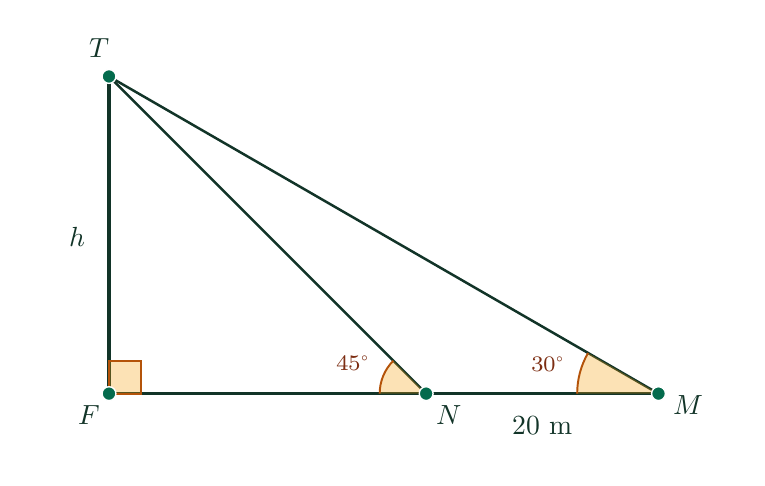
\begin{tikzpicture}[x=0.7377cm, y=0.7377cm]
\tkzDefPoint(0,5.46){T}
\tkzDefPoint(0,0){F}
\tkzDefPoint(5.46,0){N}
\tkzDefPoint(9.46,0){M}
\begin{scope}
\clip (-1.4,-1.1) rectangle (10.8,6.3);
\tkzDrawSegment[draw=ink, line width=1.80pt](F,T)
\tkzDrawSegment[draw=ink, line width=0.90pt](F,M)
\tkzDrawSegment[draw=ink, line width=0.90pt](T,N)
\tkzDrawSegment[draw=ink, line width=0.90pt](T,M)
\end{scope}
\tkzMarkRightAngle[size=0.41, draw={rgb,255:red,180;green,83;blue,9}, line width=0.7pt, fill={rgb,255:red,245;green,158;blue,11}, fill opacity=0.3](N,F,T)
\tkzFillAngle[size=1.4, fill={rgb,255:red,245;green,158;blue,11}, fill opacity=0.3](T,M,F)
\tkzMarkAngle[size=1.4, draw={rgb,255:red,180;green,83;blue,9}, line width=0.7pt, mark=none](T,M,F)
\tkzLabelAngle[pos=1.969, text={rgb,255:red,124;green,45;blue,18}, font=\footnotesize](T,M,F){$30^\circ$}
\tkzFillAngle[size=0.8, fill={rgb,255:red,245;green,158;blue,11}, fill opacity=0.3](T,N,F)
\tkzMarkAngle[size=0.8, draw={rgb,255:red,180;green,83;blue,9}, line width=0.7pt, mark=none](T,N,F)
\tkzLabelAngle[pos=1.369, text={rgb,255:red,124;green,45;blue,18}, font=\footnotesize](T,N,F){$45^\circ$}
\node[dot, fill={rgb,255:red,4;green,107;blue,77}] at (T) {};
\node[dot, fill={rgb,255:red,4;green,107;blue,77}] at (F) {};
\node[dot, fill={rgb,255:red,4;green,107;blue,77}] at (N) {};
\node[dot, fill={rgb,255:red,4;green,107;blue,77}] at (M) {};
\node[lab, font=\normalsize] at (7.46,-0.55) {$20\text{ m}$};
\node[lab, font=\normalsize] at (-0.55,2.7) {$h$};
\node[lab, font=\normalsize, anchor=center, xshift=-4.21pt, yshift=10.16pt] at (0,5.46) {$T$};
\node[lab, font=\normalsize, anchor=center, xshift=-7.78pt, yshift=-7.78pt] at (0,0) {$F$};
\node[lab, font=\normalsize, anchor=center, xshift=7.78pt, yshift=-7.78pt] at (5.46,0) {$N$};
\node[lab, font=\normalsize, anchor=center, xshift=10.16pt, yshift=-4.21pt] at (9.46,0) {$M$};
\end{tikzpicture}
\end{document}
